Avant toute explication, voici le schéma muni d’annotations afin d’identifier plus facilement chaque élément matériel.\\

\begin{figure}[H]
    \begin{center}
        \frame{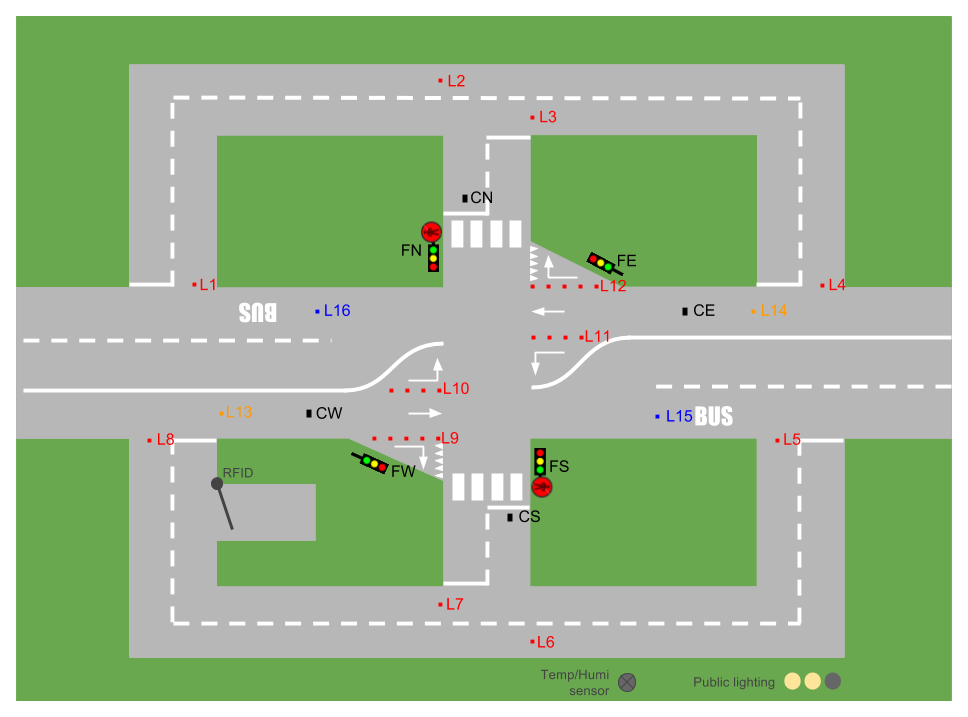
\includegraphics[width=\linewidth, height=\textheight,keepaspectratio]{img/maquette-materiel}}

        \caption{Croquis de la maquette}
    \end{center}
\end{figure}

La partie hardware sera divisée en deux parties principales. Dans un premier temps, l’arduino et l’ensemble des capteurs, des leds et des affichages lui étant connectés seront abordées. Deuxièmement, l’ensemble des interfaces Phidgets vous seront détaillées, évidemment les précisions les plus précises seront apportées à l’InterfaceKit 8/8/8 qui a recueilli une multitude de capteurs et de leds.\\

\subsection{Arduino}
\subsubsection{Élément connectés}
\subsubsection{Détails techniques}

\subsection{Phidgets}
\subsubsection{InterfaceKit 8/8/8}
\subsubsection{Advanced Servo 1-Motor}
\subsubsection{RFID Read-Write}

